%% Преамбула TeX-файла

% 1. Стиль и язык
\documentclass[utf8x, 14pt]{G7-32} % Стиль (по умолчанию будет 14pt)

% Остальные стандартные настройки убраны в preamble.inc.tex.
\sloppy

% Настройки стиля ГОСТ 7-32
% Для начала определяем, хотим мы или нет, чтобы рисунки и таблицы нумеровались в пределах раздела, или нам нужна сквозная нумерация.
\EqInChapter % формулы будут нумероваться в пределах раздела
\TableInChapter % таблицы будут нумероваться в пределах раздела
\PicInChapter % рисунки будут нумероваться в пределах раздела

% Добавляем гипертекстовое оглавление в PDF
\usepackage[
bookmarks=true, colorlinks=true, unicode=true,
urlcolor=black,linkcolor=black, anchorcolor=black,
citecolor=black, menucolor=black, filecolor=black,
]{hyperref}
\usepackage{pgfplots}
\usepackage{nomencl}

\usepackage{float}

\AfterHyperrefFix

\usepackage{microtype}% полезный пакет для микротипографии, увы под xelatex мало чего умеет, но под pdflatex хорошо улучшает читаемость
\usepackage{indentfirst}

% Тире могут быть невидимы в Adobe Reader
\ifInvisibleDashes
\MakeDashesBold
\fi

\usepackage{graphicx}   % Пакет для включения рисунков

% С такими оно полями оно работает по-умолчанию:
% \RequirePackage[left=20mm,right=10mm,top=20mm,bottom=20mm,headsep=0pt,includefoot]{geometry}
% Если вас тошнит от поля в 10мм --- увеличивайте до 20-ти, ну и про переплёт не забывайте:
\geometry{right=10mm}
\geometry{left=30mm}
\geometry{bottom=20mm}
\geometry{ignorefoot}% считать от нижней границы текста


% Пакет Tikz
\usepackage{tikz}
\usetikzlibrary{arrows,positioning,shadows}

% Произвольная нумерация списков.
\usepackage{enumerate}

% ячейки в несколько строчек
\usepackage{multirow}

% itemize внутри tabular
\usepackage{paralist,array}

%\setlength{\parskip}{1ex plus0.5ex minus0.5ex} % разрыв между абзацами
\setlength{\parskip}{1ex} % разрыв между абзацами
\usepackage{blindtext}

% Центрирование подписей к плавающим окружениям
%\usepackage[justification=centering]{caption}

\usepackage{newfloat}
\DeclareFloatingEnvironment[
placement={!ht},
name=Equation
]{eqndescNoIndent}
\edef\fixEqndesc{\noexpand\setlength{\noexpand\parindent}{\the\parindent}\noexpand\setlength{\noexpand\parskip}{\the\parskip}}
\newenvironment{eqndesc}[1][!ht]{%
    \begin{eqndescNoIndent}[#1]%
\fixEqndesc%
}
{\end{eqndescNoIndent}}

\usepackage{afterpage}

\newcommand\blankpage{
	\null
	\thispagestyle{empty}
	\newpage
}



% Настройки листингов.
\ifPDFTeX
% 8 Листинги

\usepackage{listings}

% Значения по умолчанию
\lstset{
  basicstyle= \footnotesize,
  breakatwhitespace=true,% разрыв строк только на whitespacce
  breaklines=true,       % переносить длинные строки
%   captionpos=b,          % подписи снизу -- вроде не надо
  inputencoding=koi8-r,
  numbers=left,          % нумерация слева
  numberstyle=\footnotesize,
  showspaces=false,      % показывать пробелы подчеркиваниями -- идиотизм 70-х годов
  showstringspaces=false,
  showtabs=false,        % и табы тоже
  stepnumber=1,
  tabsize=4,              % кому нужны табы по 8 символов?
  frame=single,
  xleftmargin=2.4em,
  framexleftmargin=2em
}

% Стиль для псевдокода: строчки обычно короткие, поэтому размер шрифта побольше
\lstdefinestyle{pseudocode}{
  basicstyle=\small,
  keywordstyle=\color{black}\bfseries\underbar,
  language=Pseudocode,
  numberstyle=\footnotesize,
  commentstyle=\footnotesize\it
}

% Стиль для обычного кода: маленький шрифт
\lstdefinestyle{realcode}{
  basicstyle=\scriptsize,
  numberstyle=\footnotesize
}

% Стиль для коротких кусков обычного кода: средний шрифт
\lstdefinestyle{simplecode}{
  basicstyle=\footnotesize,
  numberstyle=\footnotesize
}

% Стиль для BNF
\lstdefinestyle{grammar}{
  basicstyle=\footnotesize,
  numberstyle=\footnotesize,
  stringstyle=\bfseries\ttfamily,
  language=BNF
}

% Определим свой язык для написания псевдокодов на основе Python
\lstdefinelanguage[]{Pseudocode}[]{Python}{
  morekeywords={each,empty,wait,do},% ключевые слова добавлять сюда
  morecomment=[s]{\{}{\}},% комменты {а-ля Pascal} смотрятся нагляднее
  literate=% а сюда добавлять операторы, которые хотите отображать как мат. символы
    {->}{\ensuremath{$\rightarrow$}~}2%
    {<-}{\ensuremath{$\leftarrow$}~}2%
    {:=}{\ensuremath{$\leftarrow$}~}2%
    {<--}{\ensuremath{$\Longleftarrow$}~}2%
}[keywords,comments]

% Свой язык для задания грамматик в BNF
\lstdefinelanguage[]{BNF}[]{}{
  morekeywords={},
  morecomment=[s]{@}{@},
  morestring=[b]",%
  literate=%
    {->}{\ensuremath{$\rightarrow$}~}2%
    {*}{\ensuremath{$^*$}~}2%
    {+}{\ensuremath{$^+$}~}2%
    {|}{\ensuremath{$|$}~}2%
}[keywords,comments,strings]

% Подписи к листингам на русском языке.
\renewcommand\lstlistingname{Листинг}
\renewcommand\lstlistlistingname{Листинги}

\else
\usepackage{local-minted}
\fi

% Полезные макросы листингов.
% Любимые команды
\newcommand{\Code}[1]{\textbf{#1}}


% Стиль титульного листа и заголовки

%\NirEkz{Экз. 3}                                  % Раскоментировать если не требуется
%\NirGrif{Секретно}                % Наименование грифа

%\gosttitle{Gost7-32}       % Шаблон титульной страницы, по умолчанию будет ГОСТ 7.32-2001, 
% Варианты GostRV15-110 или Gost7-32 
 
\NirOrgLongName{ 
МОСКОВСКИЙ ГОСУДАРСТВЕННЫЙ ТЕХНИЧЕСКИЙ УНИВЕРСИТЕТ ИМ. Н. Э. БАУМАНА
}                                           %% Полное название организации

\NirUdk{УДК № 004.822}
%\NirGosNo{№ госрегистрации }
%\NirInventarNo{Инв. № ??????}

%\NirConfirm{Согласовано}                  % Смена УТВЕРЖДАЮ
\NirBoss[.49]{Проректор университета\\по научной работе}{В.Н. Зимин.}            %% Заказчик, утверждающий НИР


%\NirReportName{Научно-технический отчет}   % Можно поменять тип отчета
%\NirAbout{О составной части \par опытно-конструкторской работы} %Можно изменить о чем отчет

%\NirPartNum{Часть}{1}                      % Часть номер

%\NirBareSubject{}                  % Убирает по теме если раскоментить

% \NirIsAnnotacion{АННОТАЦИОННЫЙ }         %% Раскомментируйте, если это аннотационный отчёт
%\NirStage{промежуточный}{Этап \No 1}{} %%% Этап НИР: {номер этапа}{вид отчёта - промежуточный или заключительный}{название этапа}
%\NirStage{}{}{} %%% Этап НИР: {номер этапа}{вид отчёта - промежуточный или 

\Nir{}

\NirSubject{Драйвер нулевого уровня для использования графического планшета в качестве клавиатуры}                % Наименование темы
%\NirFinal{}                        % Заключительный, если закоментировать то промежуточный
%\finalname{итоговый}               % Название финального отчета (Заключительный)
%\NirCode{Шифр\,---\,САПР-РЛС-ФИЗТЕХ-1} % Можно задать шифр как в ГОСТ 15.110
\NirCode{}

% \NirManager{Зам. проректора по научной работе}{Р.А. Бадамшин  } %% Название руководителя
\NirIsp{Руководитель темы}{Кирилл Леонидович Тассов} %% Название руководителя

\NirYear{2020}%% если нужно поменять год отчёта; если закомментировано, ставится текущий год
\NirTown{Москва}                           %% город, в котором написан отчёт


\usepackage{pdfpages}

\begin{document}

\frontmatter % выключает нумерацию ВСЕГО; здесь начинаются ненумерованные главы: реферат, введение, глоссарий, сокращения и прочее.

%\maketitle %создает титульную страницу

\includepdf[pages=-]{pages/title.pdf}
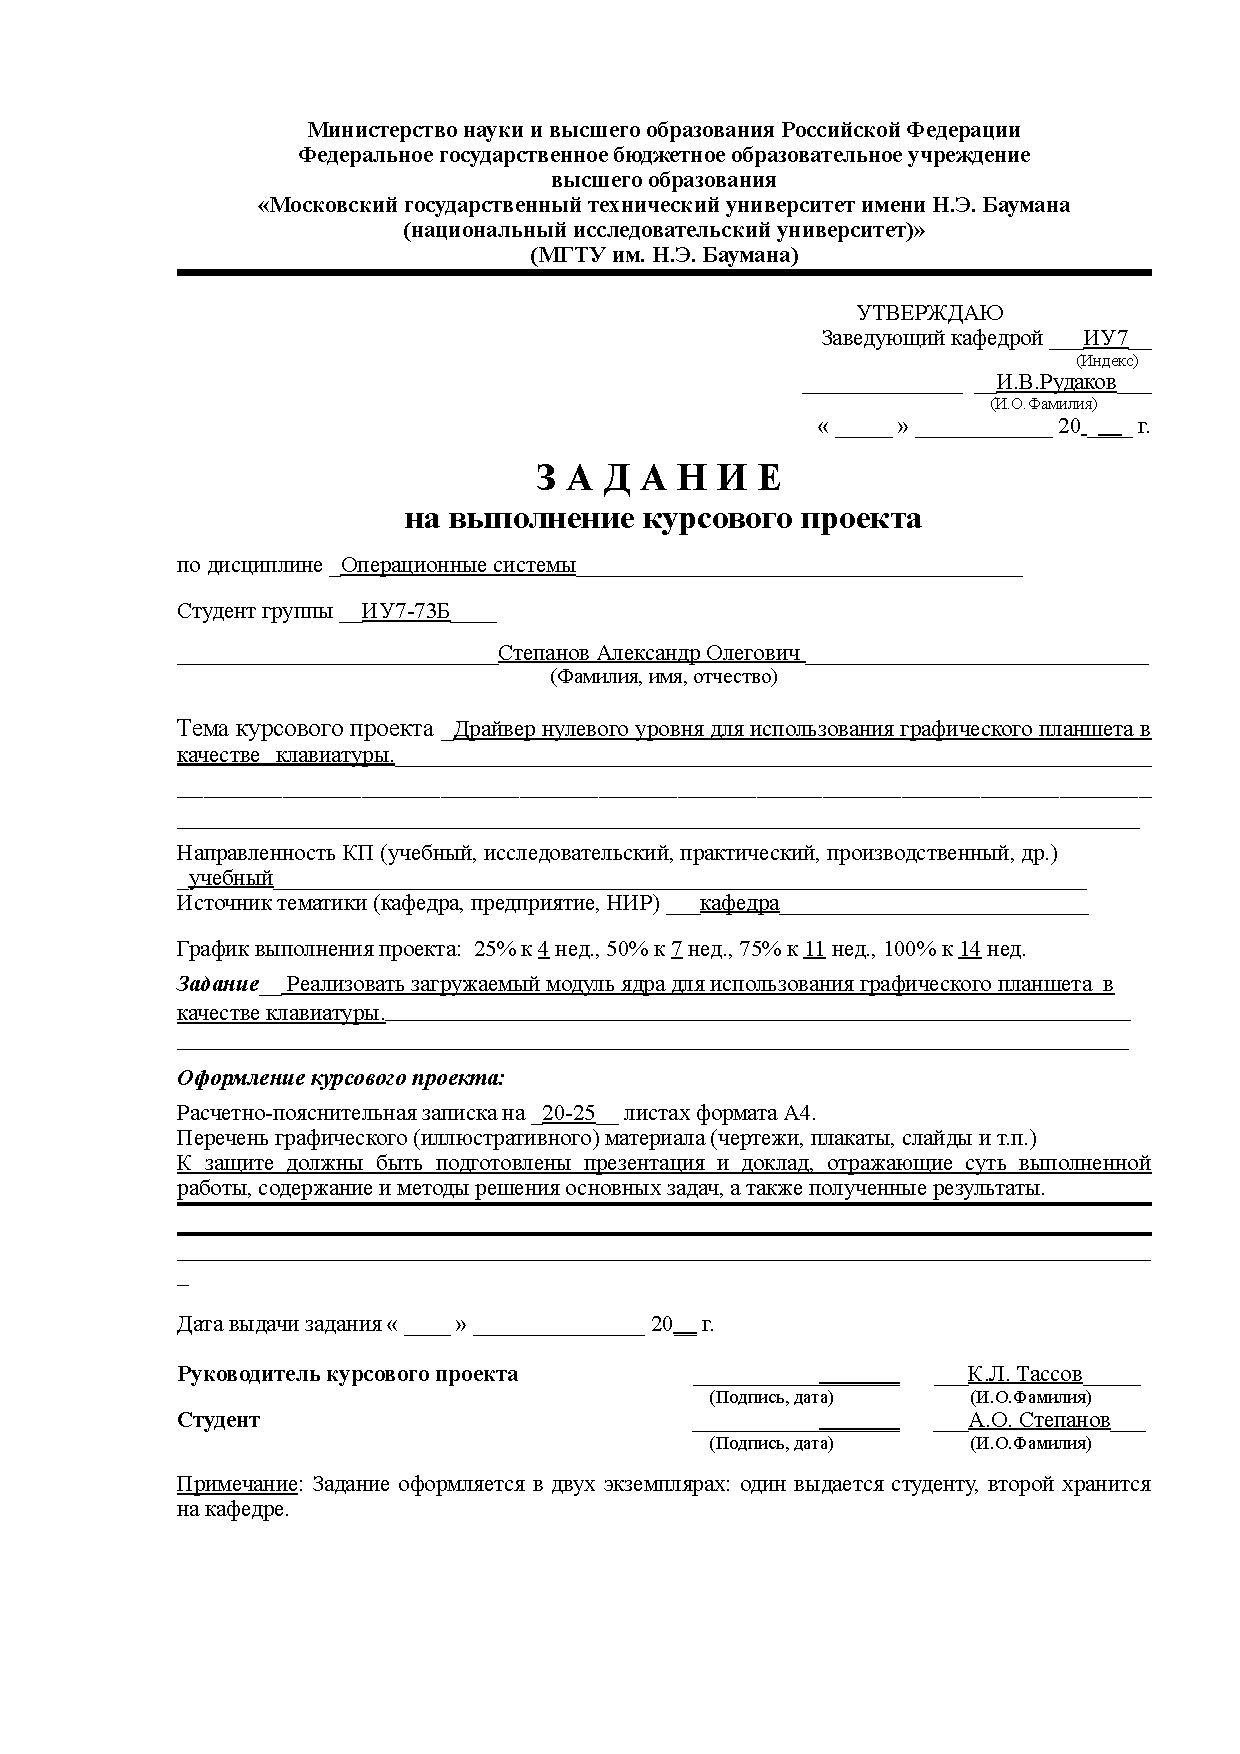
\includepdf[pages=-]{pages/tz.pdf}
% пропущены страницы под тз и план (у меня их 2 тз и 1 план, итого 3, вам надо пропустить столько, сколько страниц у вас в тз и плане)


%\listoffigures                         % Список рисунков

%\listoftables                          % Список таблиц

%\NormRefs % Нормативные ссылки 
% Команды \breakingbeforechapters и \nonbreakingbeforechapters
% управляют разрывом страницы перед главами.
% По-умолчанию страница разрывается.

\Referat
%\begin{abstract}

    Отчет содержит \pageref{LastPage}\,стр.%
    \ifnum \totfig >0
    , \totfig~рис.%
    \fi
    \ifnum \tottab >0
    , \tottab~табл.%
    \fi
    %
    \ifnum \totbib >0
    , \totbib~источн.%
    \fi
    %
    \ifnum \totapp >0
    , \totapp~прил.%
    \else
    .%
    \fi

    Ключевые слова: linux, драйвер, графический планшет, загружаемый модуль ядра, клавиатура, прерывания, пространство ядра.

    Курсовой проект представляет собой загружаемый модуль ядра для использования графического планшета в качестве клавиатуры. Используется язык программирования C.

%\end{abstract}

%%% Local Variables:
%%% mode: latex
%%% TeX-master: "rpz"
%%% End:

% \nobreakingbeforechapters
% \breakingbeforechapters

\tableofcontents

% \printnomenclature % Автоматический список сокращений

\Introduction

В настоящее время невозможно представить работу за компьютером без полноценной клавиатуры, но не всегда имеется возможность взять с собой такое большое устройство. Одним из самых мобильных и небольших устройств, которое похоже на клавиатуру, является графический планшет. Графический планшет имеет плоскую форму, которую удобно взять с собой, в отличии от клавиатуры. Поэтому существует потребность создания драйвера для использования графического планшета в качестве клавиатуры.

Целью данной работы является разработка загружаемого модуля ядра для эмитации работы клавиатуры на графическом планшете.

Для достижения этой цели ставятся следующие задачи:

\begin{enumerate}
    \item изучение подходов для реализации драйвера устройства linux;
    \item изучение подходов для эмитации работы клавиатуры;
    \item реализация требуемого драйвера нулевого уровня.
\end{enumerate}


\mainmatter % это включает нумерацию глав и секций в документе ниже

\chapter{Аналитический раздел}
\label{cha:analysis}

Требуется разработать драйвер для графического планшета, позволяющий работать устройству в качестве клавиатуры. В данном разделе рассматриваются методы решения поставленной задачи.

\section{Графический планшет}

Графический планшет -- это устройство для ввода информации, созданной от руки, непосредственно в компьютер. Состоит из пера (стилуса) и плоского планшета, чувствительного к нажатию или близости пера.

Для разработки и тестирования данной работы используется планшет Wacom CTL-671, его изоражение представлено на рисунке \ref{fig:wacom}.

\begin{figure}[H]
    \centering
    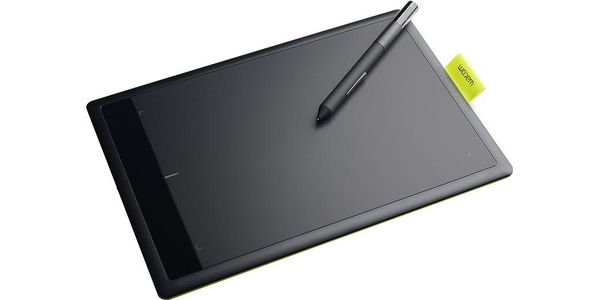
\includegraphics[width=0.8\textwidth]{img/wacom.jpg}
    \caption{Графический планшет Wacom CTL-671}
    \label{fig:wacom}
\end{figure}

\section{Загружаемый модуль ядра}

Загружаемый модуль ядра -- объектный файл, содержащий код, расширяющий возможности ядра операционной системы. Модули используются, чтобы добавить поддержку нового оборудования или файловых систем или для добавления новых системных вызовов. Когда функциональность, предоставляемая модулем, больше не требуется, он может быть выгружен, чтобы освободить память и другие ресурсы.

\subsection{Драйвер устройства}

Драйверы устройств являются одной из разновидностей модулей ядра. Они играют особую роль. Драйверы полностью скрывают детали, касающиеся рабоыт устройства и предоставляют четкий программный интерфейс для работы с аппаратурой. В Unix каждое аппаратное устройство представлено псевдофайлом (файлом устройства) в каталоге /dev. Этот файл обеспечивает средства взаимодействия с аппаратурой.

\section{Подключение графического планшета}

Первой задачей стоит подключение графического планшета для обработки прерываний при нажатии на устройство.

\subsection{Прерывания}

Прерывание -- сигнал к процессору, испускаемый аппаратными средствами или программным обеспечением, и указывающий на событие, которое требует немедленного внимания. Прерывание предупреждает процессор о высокоприоритетном состоянии, требующем прерывания текущего кода, выполняемого процессором. Процессор отвечает, приостанавливая свои текущие действия, сохраняя свое состояние и выполняя функцию, называемую обработчиком прерываний (или подпрограммой обработки прерываний, ISR) для обработки события. Это прерывание является временным, и после завершения обработки обработчика прерывания процессор возобновляет обычную работу. Существует два типа прерываний: аппаратные прерывания и программные прерывания \cite{Interrupts}.

Каждое прерывание имеет свой собственный обработчик прерываний. Количество аппаратных прерываний ограничено числом строк запроса прерывания (IRQ) для процессора, но могут быть сотни различных программных прерываний. Прерывания — это широко используемая техника многозадачности компьютеров, в первую очередь в реальном времени. Такая система называется управляемой прерываниями.

\subsection{Драйвер usb устройства}

Для того, чтобы перехватывать прерывания графического планшета необходимо создать драйвер usb устройства и подключить планшет к нему.

\subsubsection{Структура usb\_driver}

Для создания драйвера usb устройства необходимо использовать структуру usb\_driver \cite{Usb_driver}. 4 главных поля, которые необходимо использовать это: name (имя загружаемого драйвера), probe (указатель на функцию, вызывающуюся при подключении устройства), disconnect (указатель на функцию, вызывающуюся при отключении устройства) и id\_table (список устройств, которые надо автоматически подключать к драйверу, для идентификации устройства используются id поставщика устройства и id самого устройства).

\subsubsection{Работа драйвера usb устройства}

После создания экземляра структуры, представляющей из себя usb драйвер, его необходимо зарегестрировать в системе с помощью системного вызова usb\_register. Если usb драйвер будет успешно зарегестрирован, то он попытается подключить все подходящие устройства, подключенные к системе и незанятые никаким драйвером. Выбор устройств для попытки подключения делается с помощью поля id\_table. Если функция подключения вернет код успешного завершения, то устройство будет подключено к драйверу \cite{Usb_driver}.

\subsubsection{Подключение графического планшета}

Для подключения планшета в функции probe необходимо проделать следующую последовательность действий:

\begin{itemize}
    \item выделить память для экземпляра структуры планшета;
    \item выделить память для устройства ввода;
    \item выделить память для URB (USB Request Block);
    \item получить свободный путь в файловой системе для устройства ввода;
    \item связать прерывание устройства с функцией;
    \item зарегистрировать устройство.
\end{itemize}

\subsection{Многозадачность для прерываний}

Чтобы сократить время выполнения обработчиков прерываний обработчики медленных аппаратных прерываний делятся на две части, которые традиционно называются верхняя (top) и нижняя (bottom) половины (half). Верхними половинами остаются обработчики, устанавливаемы функцией request\_irq() на определенных IRQ. Выполнение нижних половин инициируется верхними половинами, т.е. обработчиками прерываний \cite{BottomHalf}.

В ОС Linux имеется три типа нижних половин (bottom half) \cite{BottomHalf}:

\begin{itemize}
    \item softirq -- отложенные прерывания;
    \item tascklet -- тасклеты;
    \item workqueue -- очереди работ.
\end{itemize}

Для обработки прерываний испольуют тасклеты и очереди работ. Рассмотрим данные методы.

\subsubsection{Тасклеты}

Тасклеты -- это механизм обработки нижних половин, построенный на основе механизма отложенных прерываний \cite{BottomHalf}.

Тасклеты описываются следующей структурой, описанной на листинге \ref{lst:tasklet} \cite{Tasklets}.

\begin{lstlisting}[language=c,caption=Структура tasklet,label=lst:tasklet]
struct tasklet_struct
{
    struct tasklet_struct *next;
    unsigned long state;
    atomic_t count;
    void (*func)(unsigned long);
    unsigned long data;
};
\end{lstlisting}

В данной структуре имеются поля \cite{Tasklets}:

\begin{itemize}
    \item next -- указатель на следюущий тасклет в списке;
    \item state -- состояние тасклета;
    \item func -- функция обработчик тасклета;
    \item data -- аргумент функции обработчика тасклета.
\end{itemize}

Когда tasklet запланирован, он добавляется в очередь. Пока он находится в этом состоянии, запланировать его еще раз не получится -- в этом случае просто ничего не произойдет. Tasklet не может находиться сразу в нескольких местах в очереди на планирование, которая организуется через поле next структуры tasklet\_struct. После того, как тасклет был запланирован, он выполнится один раз \cite{Tasklets}.

\subsubsection{Очереди работ}

Очередь работ является еще одной концепцией для обработки отложенных функций. Функции рабочих очередей выполняются в контексте процесса ядра. Это означает, что функции очереди задач не должны быть атомарными, как функции тасклета. Подсистема рабочей очереди представляет собой интерфейс для создания потоков ядра для обработки работы (work), которая ставится в очередь. Такие потоки ядра называются рабочими потоками. Рабочая очередь поддерживается типом struct work\_struct, описанным на листинге \ref{lst:work_struct} \cite{WorkQueue}.

\begin{lstlisting}[language=c,caption=Структура work\_struct,label=lst:work_struct]
struct work_struct
{
    atomic_long_t data;
    struct list_head entry;
    work_func_t func;
# ifdef CONFIG_LOCKDEP
    struct lockdep_map lockdep_map;
# endif
};
\end{lstlisting}

Очередь работ создается функцией:

\begin{lstlisting}[language=c]
int create_workqueue(char *name, unsigned int flags, int max_active);
\end{lstlisting}

\begin{itemize}
    \item name -- имя очереди, но в отличие от старых реализаций потоков с этим именем не создается;
    \item flags -- флаги определяют как очередь работ будет выполняться;
    \item max\_active -- ограничивает число задач из данной очереди, которые могут одновременно выполняться на одном CPU.
\end{itemize}

Для того, чтобы поместить задачу в очередь работ надо заполнить (инициализировать) структуру work\_struct.

После того, как работа была создана, следующим шагом будет помещение этой структуры в очередь работ. Это можно сделать несколькими способами. Во-первых, просто добавить работу (объект work) в очередь работ с помощью функции queue\_work (которая назначает работу текущему процессору). Можно с помощью функции queue\_work\_on указать процессор, на котором будет выполняться обработчик.
Две дополнительные функции обеспечивают те же функции для отложенной работы (в которой инкапсулирована структура work\_struct и таймер, определяющий задержку): queue\_delayed\_work, queue\_delayed\_work\_on \cite{WorkQueue}.

Кроме того, можно использовать глобальное ядро -- глобальную очередь работ с четырьмя функциями, которые работают с этой очередью работ. Эти функции имитируют предыдущие функции, за исключением лишь того, что не нужно определять структуру очереди работ \cite{WorkQueue}.

\section{Работа клавиатуры}

Для эмуляции работы клавиатуры необходимо вызывать нажатия клавиш после обработки прерываний графического планшета.

\subsection{Подсистема ввода/вывода}

Подсистема ввода/вывода выполняет запросы файловой подсистемы и подсистемы управления процессами для доступа к периферийным устройствам (дискам, магнитным лентам, терминалам и т.д.). Она обеспечивает необходимую буферизацию данных и взаимодействует с драйверами устройств — специальными модулями ядра, непосредственно обслуживающими внешние устройства \cite{Subsystem}.

Подсистемой ввода/вывода поддерживаются три вида устройств:

\begin{itemize}
    \item символьные устройства для поддержки последовательных устройств;
    \item блочные устройства для поддержки устройств с произвольным доступом, блочные устройства имеют важное значение для реализации файловых систем;
    \item сетевые устройства, которые поддерживают широкий спектр устройств на канальном уровне.
\end{itemize}

Для использования подсистемы ввода/вывода используется структура input\_dev \cite{Input_dev}. Чтобы инициализировать эту структуру используется функция set\_bit, которая принимает два аргумента: бит, который устанавливается, и адрес, куда этот бит устанавливать \cite{Setbit}.

\subsubsection{Установка событий}

Для установки типа события, которое будет вызываться необходимо установить бит EV\_KEY \cite{EVkey} в поле evbit в структуре input\_dev \cite{Input_dev}. После установки бита события устанавливаются биты клавиш, которые будут вызываться, например, KEY\_0 (клавиша с цифрой 0), KEY\_Z (клавиша с буквой z) и KEY\_CAPSLOCK (клавиша CapsLock).

\subsubsection{Вызов событий}

Для вызова событий, связанных с клавишами используется системный вызов input\_report\_key \cite{Input_report_key}, который принимает устройство ввода (структура input\_dev), клавишу, на которую вызывается событие, и код события. В данной работе необходимы два кода событий: 1 -- кнопка зажата, 0 -- кнопка отжата.

\section{Вывод}

Таким образом были рассмотрены методы решения задачи разработки драйвера нулевого уровня для использования графического планшета в качестве клавиатуры.

\chapter{Конструкторский раздел}
\label{cha:design}

В данном разделе рассматривается структура программного обеспечения.

\section{Состав программного обеспечения}

Программное обеспечение состоит из загружаемого модуля ядра.

\subsection{Загрузка модуля ядра}

Для компиляции модуля используется специальный makefile. На листинге \ref{lst:make} представлен makefile, с помощью которого компилировался модуль ядра из данной работы.

\begin{lstlisting}[language=make,caption=Makefile для компиляции модуля ядра,label=lst:make]
ifneq ($(KERNELRELEASE),)
    obj-m := keyboard_tablet.o
else
    CURRENT = $(shell uname -r)
    KDIR = /lib/modules/$(CURRENT)/build
    PWD = $(shell pwd)

all:
    $(MAKE) -C $(KDIR) M=$(PWD) modules

clean:
    @rm -f *.o .*.cmd .*.flags *.mod.c *.order
    @rm -f .*.*.cmd *~ *.*~ TODO.*
    @rm -fR .tmp*
    @rm -rf .tmp_versions

disclean: clean
    @rm *.ko *.symvers

endif
\end{lstlisting}

После компиляции получается объектный файл с расширением .ko, который можно загрузить в ядро с помощью команды insmod под sudo.

\section{Создание usb драйвера}

Для создания usb драйвера создается экземпляр структуры usb\_driver \cite{Usb_driver}. Создание экземпляра приведено на листинге \ref{lst:usb_driver}.

\begin{lstlisting}[language=c,caption=Создание экземпляра usb драйвера,label=lst:usb_driver]
static struct usb_driver tablet_driver = {
    .name       = DRIVER_NAME,
    .probe      = tablet_probe,
    .disconnect = tablet_disconnect,
    .id_table   = tablet_table,
};
\end{lstlisting}

Для ругистрации usb драйвера используется системный вызов usb\_register \cite{Usb_register}.

\section{Структура для хранения ифнормации о графическом планшете}

Для передачи данных, связанных с графическим планшетом была создана структура tablet, приведенная на листинге \ref{lst:tablet_t}.

\begin{lstlisting}[language=c,caption=Структура планшета,label=lst:tablet_t]
struct tablet {
    unsigned char     *data;
    struct input_dev  *input_dev;
    struct usb_device *usb_dev;
    struct urb        *irq;
};
typedef struct tablet tablet_t;
\end{lstlisting}

В данной структуре созданы следующие поля:

\begin{itemize}
    \item data -- данные, передаваемые планшетом при прерывании;
    \item input\_dev -- подключенный планшет;
    \item usb\_dev -- представление usb устройства;
    \item irq -- обработчик прерываний.
\end{itemize}

\section{Структура для передачи данных о прерывании}

Для того, чтобы передавать в работу из очереди данные о прерывании была создана структура container\_urb, представленная на листинге \ref{lst:container_urb}.

\begin{lstlisting}[language=c,caption=Структура для передачи данных о прерывании,label=lst:container_urb]
struct container_urb {
    struct urb *urb;
    struct work_struct work;
};

typedef struct container_urb container_urb_t;
\end{lstlisting}

В данной структуре созданы следующие поля:

\begin{itemize}
    \item urb -- обработанное прерывание;
    \item work -- текущая работа в очереди.
\end{itemize}

\section{Обработка прерываний}

На рисунке \ref{fig:urb} предствалена схема обработки прерываний графического планшета и отправка событий нажатия на клавиши клавиатуры.

\begin{figure}[H]
    \centering
    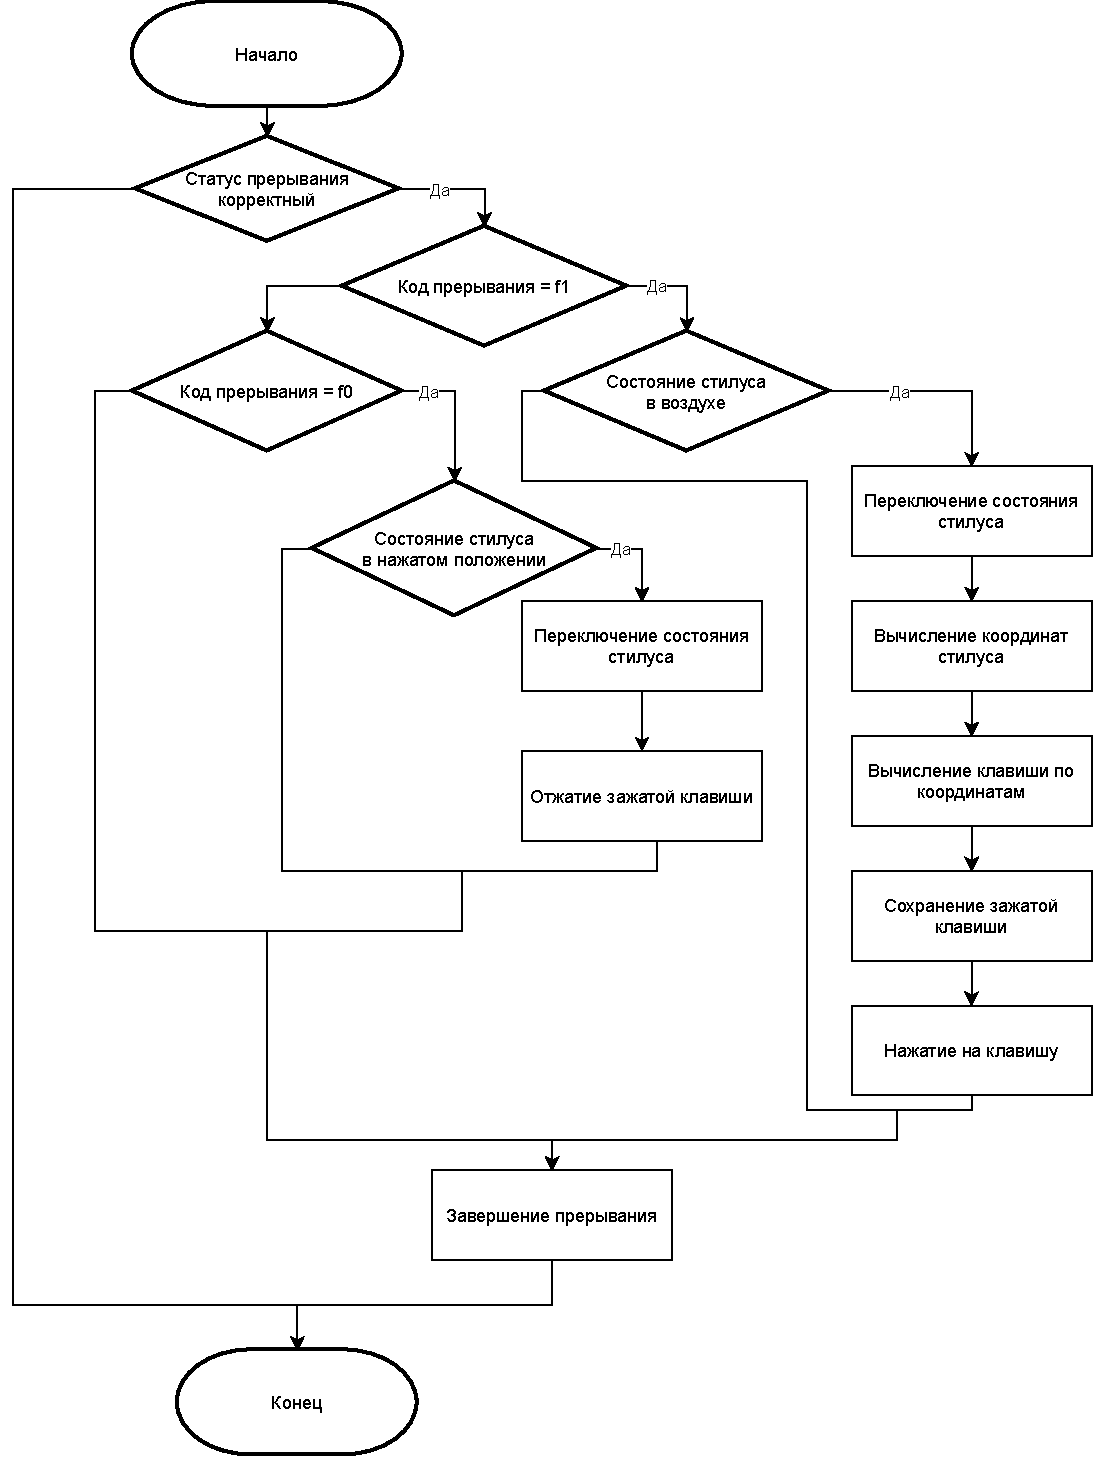
\includegraphics[width=0.9\textwidth]{img/urb.pdf}
    \caption{Обработка прерываний}
    \label{fig:urb}
\end{figure}

\section{Разделение поверхности планшета на клавиши}

Для комфортного использования модуля клавиши были расставлены на основе классической qwerty раскладки \cite{Qwerty}.

Координаты стилуса находятся в диапазоне от 0 до 1344 по оси x и от 0 до 468 по y. Поскольку координаты стилуса принимают только значения кратные 16 для оси x и кратные 9 для y, то поверхость была поделена на области размером 16 на 9. Таких областей получилось 84 на 52. Именно координаты этих областей и используются для вычисления клавиши. На рисунке \ref{fig:keyboard} представлена схема разделения поверхности планшета на клавиши клавиатуры.

\begin{figure}[H]
    \centering
    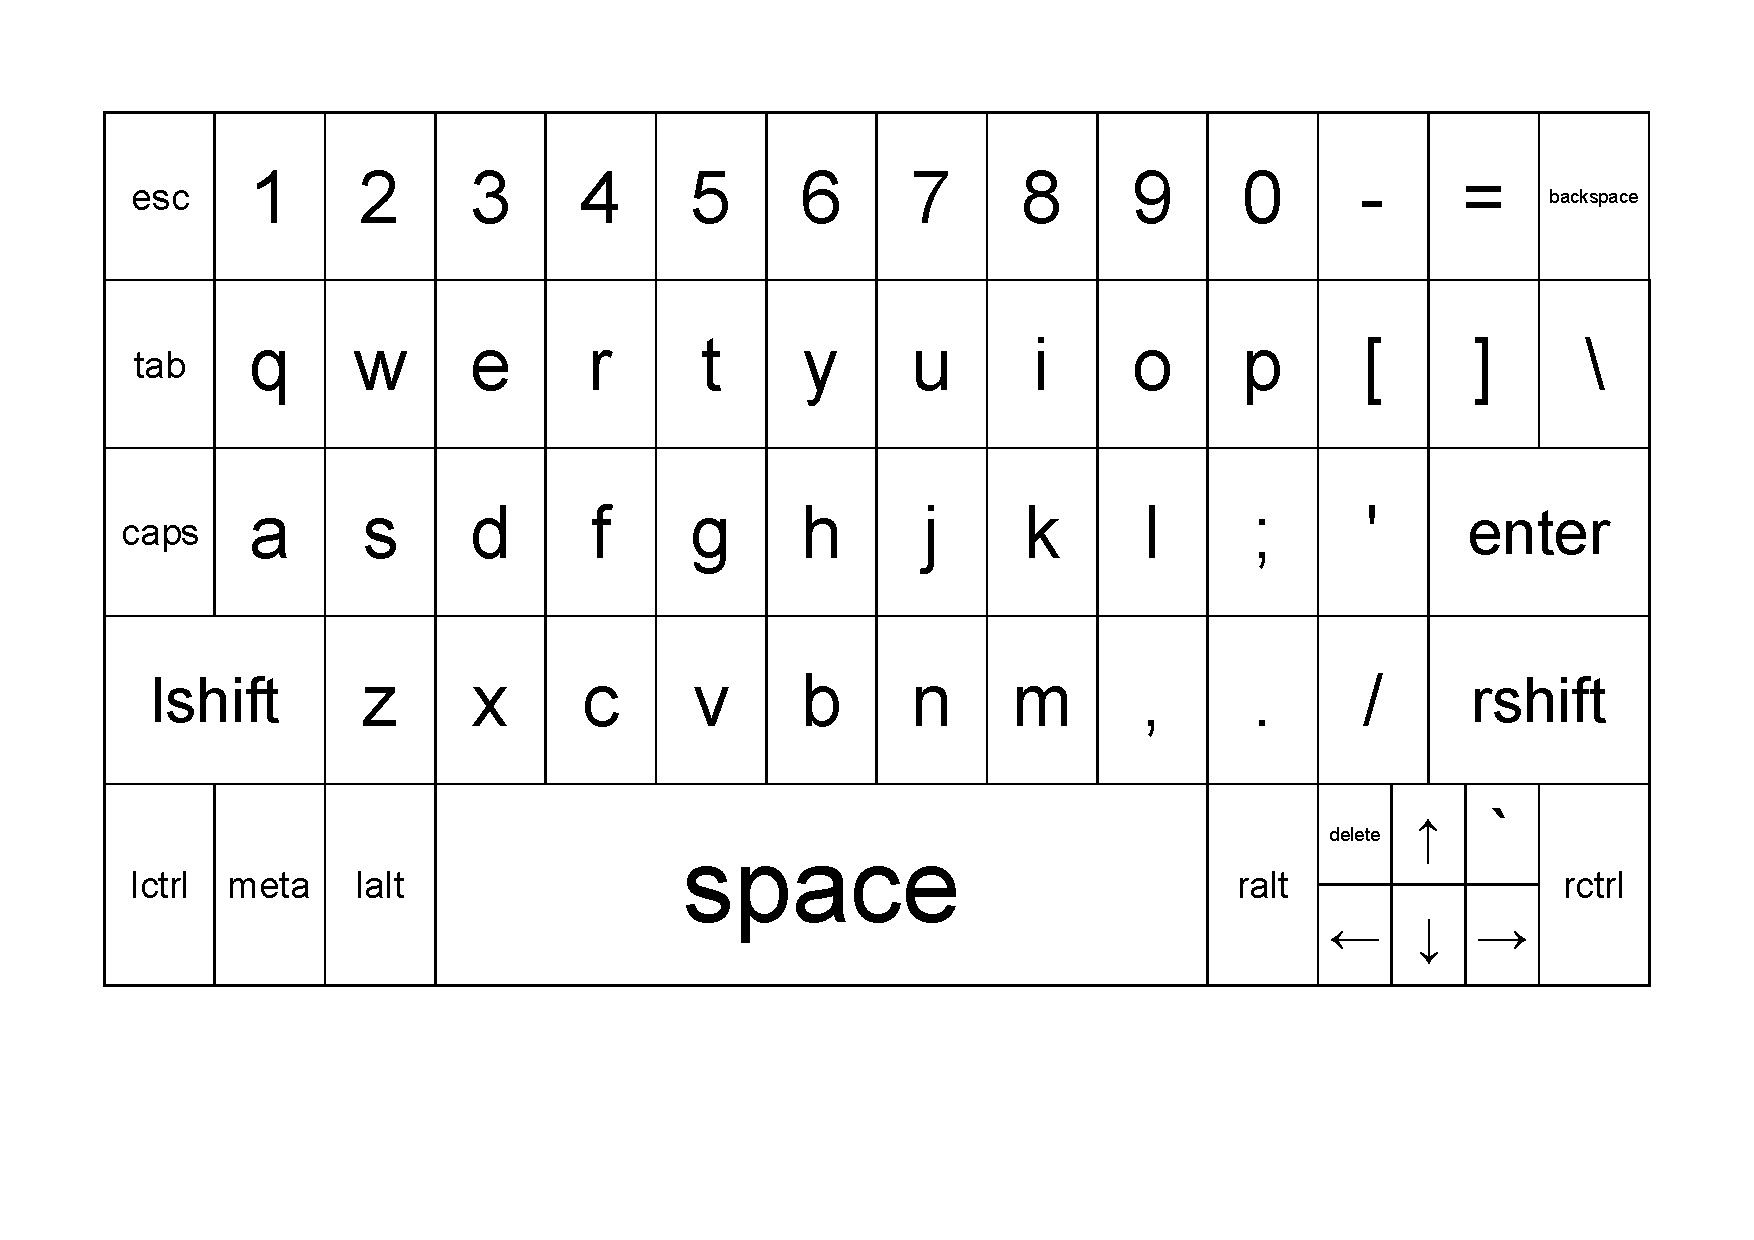
\includegraphics[trim=3cm 4cm 3cm 1.5cm, width=0.9\textwidth]{img/keyboard.pdf}
    \caption{Разделение поверхности планшета на клавиши}
    \label{fig:keyboard}
\end{figure}

\section{Вывод}

В данном разделе был рассмотрен процесс проектирования структуры программного обеспечения.

\chapter{Технологический раздел}
\label{cha:impl}

В данном разделе производится выбор средств для разработки и рассматривается реализация программного обеспечения.

\section{Выбор языка программирования}

В качестве языка программирования был выбран язык C. На этом языке реализованы все модули ядра и драйверы операционной системы Linux. Компилятор -- gcc.

\section{Работа программы}

Рассмотрим работу модуля с листингами.

\subsection{Начальная настройка}

На листинге \ref{lst:macros} представлено объявление всех необходимых макросов. На листинге \ref{lst:structs} представлено объявление всех глобальных пременных, а именно:

\begin{itemize}
    \item pen\_enter -- положение стилуса (на планшете или в воздухе);
    \item pressed\_key -- нажатая в текущий момент клавиша;
    \item workq -- очередь работ;
    \item keyboard -- виртуальное устрйоство для вывода событий клавиш.
\end{itemize}

Также там объявляются структуры tablet, которая нужна для хранения данных о состоянии планшета, и container\_urb, которая нужна для передачи данных о текущем прерывании в работу.

На листинге \ref{lst:init} представлена функция инициализации модуля, где происходит регистрация драйвера, инициализацяи очереди работ, настройка виртуального устройства клавиатуры и ее регистрация.

На листинге \ref{lst:exit} представлена функция выгрузки модуля, где происходит очистка памяти, выключение драйвера и удаление вртуального устройства.

\subsection{Драйвер для планшета}

На листинге \ref{lst:probe} представлена функция подключения планшета, в которой производится все необходимое выделение памяти и настрйока.

На листинге \ref{lst:input_dev_open_close} представлены функции открытия и закрытия устройства ввода.

На листинге \ref{lst:disconnect} представлена функция отключения планшета, в которой освобождается память и удаляются обработчики.

На листинге \ref{lst:device_id} представлена таблица устройств, которые необходимо подключать. Первый элемент этой таблицы это планшет Wacom Ltd CTL-671, который использовался для тестирования драйвера, а второй -- пустой элемент, это означает, что если нет устройства, у которого совпадают идентификаторы из других элементов таблицы, то драйвер будет пытаться подключить каждое свободное устройство.

На листинге \ref{lst:irq} представлена функция, которая перехватывает прерывание. В ней создается работа и отправляется в очередь обработки.

На листинге \ref{lst:work_irq} представлена функция, обрабатывающая прерывание. Ее алгоритм представлен на рисунке \ref{fig:urb}.

\subsection{Нажатие клавиш клавиатуры}

На листинге \ref{lst:keydown_keyup} представлены функции нажатия и отжатия текущей клавиши.

На листинге \ref{lst:press_key} представлена часть функции выбора клавиши в зависимости от координат. Разделение поверхности планшета на клавиши представлено на рисунке \ref{fig:keyboard}.

\section{Пример работы программы}

На рисунке \ref{fig:connect} изображены логи при подключении планшета в систему. В этот момент планшет также подключается и к драйверу.

\begin{figure}[H]
    \centering
    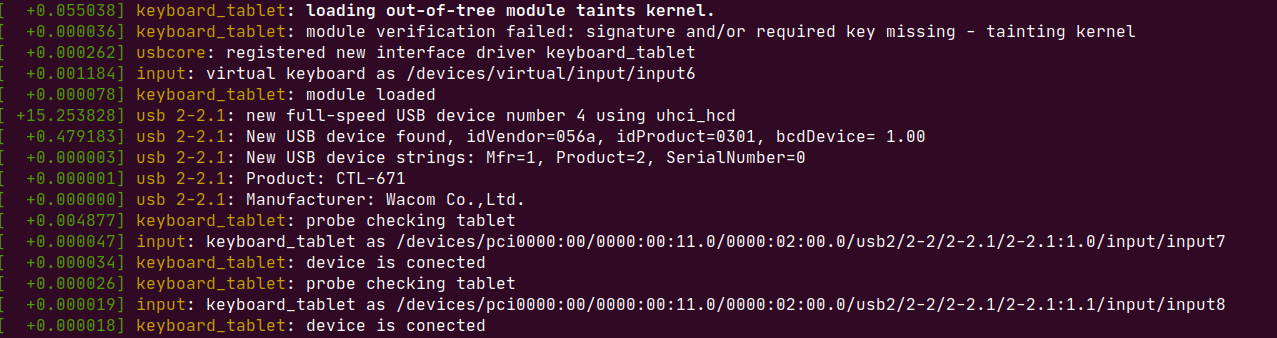
\includegraphics[width=0.8\textwidth]{img/connect.png}
    \caption{Подключение планшета к операционной системе}
    \label{fig:connect}
\end{figure}

На рисунке \ref{fig:work} изображены логи нажатий на планшет в разных областях.

\begin{figure}[H]
    \centering
    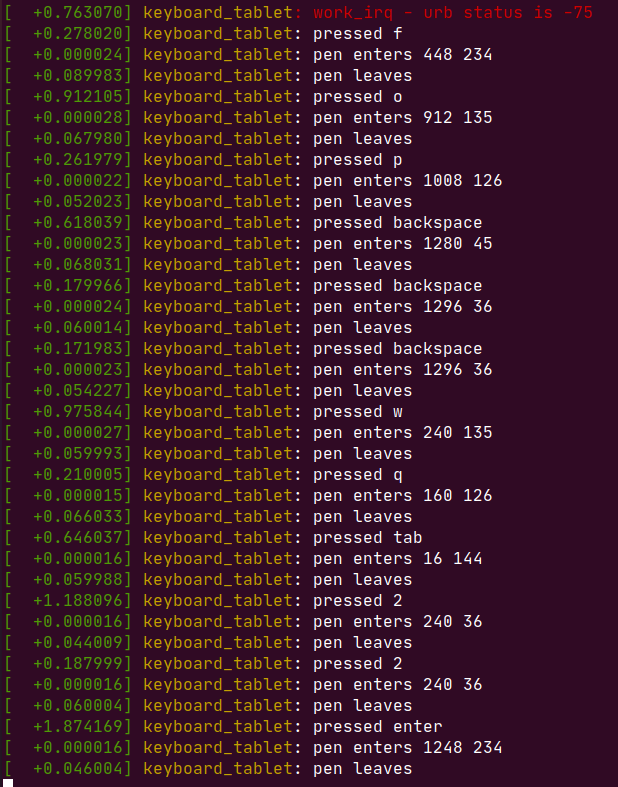
\includegraphics[width=0.8\textwidth]{img/work.png}
    \caption{Логи нажатий на планшет}
    \label{fig:work}
\end{figure}

На рисунке \ref{fig:work_wletters} изображены логи нажатий на планшет, когда открыта консоль с выводом логов. Здесь можно заметить перед сообщением о печати буквы сами эти буквы, которые были напечатаны с помощью планшета.

\begin{figure}[H]
    \centering
    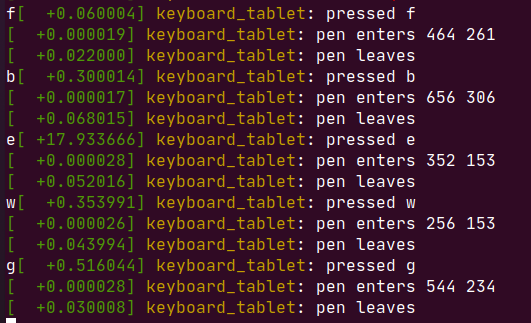
\includegraphics[width=0.8\textwidth]{img/work_wletters.png}
    \caption{Логи нажатий на планшет в консоли с логами}
    \label{fig:work_wletters}
\end{figure}

На рисунке \ref{fig:disconnect} изображены логи отключения планшета.

\begin{figure}[H]
    \centering
    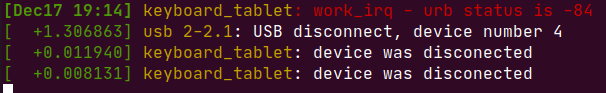
\includegraphics[width=0.8\textwidth]{img/disconnect.png}
    \caption{Отключение планшета от оперционной системы}
    \label{fig:disconnect}
\end{figure}

\section{Вывод}

В данном разделе был выбран язык программирования C, а также рассмотрена реализация программного обеспечения.

%\chapter{Исследовательский раздел}
\label{cha:research}



\backmatter %% Здесь заканчивается нумерованная часть документа и начинаются ссылки и
            
\Conclusion % заключение к отчёту

В ходе данной работы были выполнены следующие задачи:

\begin{enumerate}
    \item изучены подходы для реализации драйвера устройства linux;
    \item изучены подходы для эмитации работы клавиатуры;
    \item реализован требуемый драйвер нулевого уровня.
\end{enumerate}

Таким образом, достигнута цель реализации драйвера нулевого уровня для использования графического планшета в качестве клавиатуры на языке программирования C.
%% заключение


% % Список литературы при помощи BibTeX
% Юзать так:
%
% pdflatex rpz
% bibtex rpz
% pdflatex rpz

\bibliographystyle{ugost2008}
\bibliography{rpz}
\nocite{*}

%%% Local Variables: 
%%% mode: latex
%%% TeX-master: "rpz"
%%% End: 


%
\appendix   % Тут идут приложения
%
\chapter{Реализация}

\begin{lstlisting}[language=c,caption=Объявление начальных макросов,label=lst:macros]
#include <linux/module.h>
#include <linux/init.h>
#include <linux/kernel.h>
#include <linux/usb/input.h>
#include <linux/slab.h>
#include <linux/workqueue.h>

#define DRIVER_NAME    "keyboard_tablet"
#define DRIVER_AUTHOR  "Alexander Stepanov"
#define DRIVER_DESC    "Simulate table like a keyboard."
#define DRIVER_LICENSE "GPL"

MODULE_AUTHOR(DRIVER_AUTHOR);
MODULE_DESCRIPTION(DRIVER_DESC);
MODULE_LICENSE(DRIVER_LICENSE);

#define ID_VENDOR_TABLET  0x056a /* Wacom Co. */
#define ID_PRODUCT_TABLET 0x0301 /* Ltd CTL-671 */

#define USB_PACKET_LEN  10
#define WHEEL_THRESHOLD 4

#define MAX_X 1920
#define MAX_Y 1080

#define MAX_VALUE 0x7F

#define X_FACTOR (MAX_X / MAX_VALUE + 1)
#define Y_FACTOR (MAX_Y / MAX_VALUE + 1)
\end{lstlisting}

\begin{lstlisting}[language=c,caption=Объявление структур и глобальных переменных,label=lst:structs]
struct tablet {
    unsigned char     *data;
    dma_addr_t         data_dma;
    struct input_dev  *input_dev;
    struct usb_device *usb_dev;
    struct urb        *irq;
    int                old_wheel_pos;
    char               phys[32];
};

typedef struct tablet tablet_t;

struct container_urb {
    struct urb *urb;
    struct work_struct work;
};

typedef struct container_urb container_urb_t;

static bool pen_enter;
static int pressed_key;

static struct workqueue_struct *workq;

static struct input_dev *keyboard;

static int keys[5][14] = {
    { KEY_ESC, KEY_1, KEY_2, KEY_3, KEY_4, KEY_5, KEY_6, KEY_7, KEY_8, KEY_9, KEY_0, KEY_MINUS, KEY_EQUAL, KEY_BACKSPACE },
    { KEY_TAB, KEY_Q, KEY_W, KEY_E, KEY_R, KEY_T, KEY_Y, KEY_U, KEY_I, KEY_O, KEY_P, KEY_LEFTBRACE, KEY_RIGHTBRACE, KEY_BACKSLASH },
    { KEY_CAPSLOCK, KEY_A, KEY_S, KEY_D, KEY_F, KEY_G, KEY_H, KEY_J, KEY_K, KEY_L, KEY_SEMICOLON, KEY_APOSTROPHE, KEY_ENTER },
    { KEY_LEFTSHIFT, KEY_LEFTSHIFT, KEY_Z, KEY_X, KEY_C, KEY_V, KEY_B, KEY_N, KEY_M, KEY_COMMA, KEY_DOT, KEY_SLASH, KEY_RIGHTSHIFT, KEY_RIGHTSHIFT },
    { KEY_LEFTCTRL, KEY_LEFTMETA, KEY_LEFTALT, KEY_SPACE, KEY_SPACE, KEY_SPACE, KEY_SPACE, KEY_SPACE, KEY_SPACE, KEY_SPACE, KEY_RIGHTALT, 0, 0, KEY_RIGHTCTRL },
};

static int extra_keys[2][3] = {
    { KEY_DELETE, KEY_UP, KEY_GRAVE },
    { KEY_LEFT, KEY_DOWN, KEY_RIGHT },
};
\end{lstlisting}

\begin{lstlisting}[language=c,caption=Инициализация модуля,label=lst:init]
static int __init keyboard_tablet_init(void) {
    int result = usb_register(&tablet_driver);

    if (result < 0) {
        printk(KERN_ERR "%s: usb register error\n", DRIVER_NAME);
        return result;
    }

    workq = create_workqueue("workqueue");
    if (workq == NULL) {
        printk(KERN_ERR "%s: allocation workqueue error\n", DRIVER_NAME);
        return -1;
    }

    keyboard = input_allocate_device();
    if (keyboard == NULL) {
        printk(KERN_ERR "%s: allocation device error\n", DRIVER_NAME);
        return -1;
    }

    keyboard->name = "virtual keyboard";

    set_bit(EV_KEY, keyboard->evbit);

    for (i = 0; i < 5; ++i) {
        for (j = 0; j < 14; ++j) {
            if (keys[i][j] != 0) {
                set_bit(keys[i][j], keyboard->keybit);
            }
        }
    }

    for (i = 0; i < 2; ++i) {
        for (j = 0; j < 3; ++j) {
            set_bit(extra_keys[i][j], keyboard->keybit);
        }
    }

    result = input_register_device(keyboard);
    if (result != 0) {
        printk(KERN_ERR "%s: registration device error\n", DRIVER_NAME);
        return result;
    }

    printk(KERN_INFO "%s: module loaded\n", DRIVER_NAME);
    return 0;
}
\end{lstlisting}

\begin{lstlisting}[language=c,caption=Выгруза модуля и установка функций init и exit,label=lst:exit]
static void __exit keyboard_tablet_exit(void) {
    flush_workqueue(workq);
    destroy_workqueue(workq);
    input_unregister_device(keyboard);
    usb_deregister(&tablet_driver);
    printk(KERN_INFO "%s: module unloaded\n", DRIVER_NAME);
}

module_init(keyboard_tablet_init);
module_exit(keyboard_tablet_exit);
\end{lstlisting}

\begin{lstlisting}[language=c,caption=Объявление экземпляра usb драйвера]
static struct usb_driver tablet_driver = {
    .name       = DRIVER_NAME,
    .probe      = tablet_probe,
    .disconnect = tablet_disconnect,
    .id_table   = tablet_table,
};
\end{lstlisting}

\begin{lstlisting}[language=c,caption=Функция подключения планшета,label=lst:probe]
static int tablet_probe(struct usb_interface *interface, const struct usb_device_id *id) {
    struct usb_device *usb_device = interface_to_usbdev(interface);
    tablet_t *tablet;
    struct input_dev *input_dev;
    struct usb_endpoint_descriptor *endpoint;
    int error = -ENOMEM;

    printk(KERN_INFO "%s: probe checking tablet\n", DRIVER_NAME);

    tablet = kzalloc(sizeof(tablet_t), GFP_KERNEL);
    input_dev = input_allocate_device();
    if (!tablet || !input_dev) {
        input_free_device(input_dev);
        kfree(tablet);

        printk(KERN_ERR "%s: error when allocate device\n", DRIVER_NAME);
        return error;
    }

    tablet->data = (unsigned char *)usb_alloc_coherent(usb_device, USB_PACKET_LEN, GFP_KERNEL, &tablet->data_dma);
    if (!tablet->data) {
        input_free_device(input_dev);
        kfree(tablet);

        printk(KERN_ERR "%s: error when allocate coherent\n", DRIVER_NAME);
        return error;
    }

    tablet->irq = usb_alloc_urb(0, GFP_KERNEL);
    if (!tablet->irq) {
        usb_free_coherent(usb_device, USB_PACKET_LEN, tablet->data, tablet->data_dma);
        input_free_device(input_dev);
        kfree(tablet);

        printk(KERN_ERR "%s: error when allocate urb\n", DRIVER_NAME);
        return error;
    }

    tablet->usb_dev = usb_device;
    tablet->input_dev = input_dev;

    usb_make_path(usb_device, tablet->phys, sizeof(tablet->phys));
    strlcat(tablet->phys, "/input0", sizeof(tablet->phys));

    input_dev->name = DRIVER_NAME;
    input_dev->phys = tablet->phys;
    usb_to_input_id(usb_device, &input_dev->id);
    input_dev->dev.parent = &interface->dev;

    input_set_drvdata(input_dev, tablet);

    input_dev->open = tablet_open;
    input_dev->close = tablet_close;

    endpoint = &interface->cur_altsetting->endpoint[0].desc;

    usb_fill_int_urb(
        tablet->irq, usb_device,
        usb_rcvintpipe(usb_device, endpoint->bEndpointAddress),
        tablet->data, USB_PACKET_LEN,
        tablet_irq, tablet, endpoint->bInterval
    );

    usb_submit_urb(tablet->irq, GFP_ATOMIC);

    tablet->irq->transfer_dma = tablet->data_dma;
    tablet->irq->transfer_flags |= URB_NO_TRANSFER_DMA_MAP;

    error = input_register_device(tablet->input_dev);
    if (error) {
        usb_free_urb(tablet->irq);
        usb_free_coherent(usb_device, USB_PACKET_LEN, tablet->data, tablet->data_dma);
        input_free_device(input_dev);
        kfree(tablet);

        printk(KERN_ERR "%s: error when register device\n", DRIVER_NAME);
        return error;
    }

    usb_set_intfdata(interface, tablet);

    pen_enter = false;
    printk(KERN_INFO "%s: device is conected\n", DRIVER_NAME);

    return 0;
}
\end{lstlisting}

\begin{lstlisting}[language=c,caption=Функции открытия и закрытия устройства ввода,label=lst:input_dev_open_close]
static int tablet_open(struct input_dev *dev) {
    tablet_t *tablet = input_get_drvdata(dev);

    tablet->old_wheel_pos = -WHEEL_THRESHOLD - 1;
    tablet->irq->dev = tablet->usb_dev;
    if (usb_submit_urb(tablet->irq, GFP_KERNEL))
        return -EIO;

    return 0;
}

static void tablet_close(struct input_dev *dev) {
    tablet_t *tablet = input_get_drvdata(dev);
    usb_kill_urb(tablet->irq);
}
\end{lstlisting}

\begin{lstlisting}[language=c,caption=Функция отключения планшета,label=lst:disconnect]
static void tablet_disconnect(struct usb_interface *interface) {
    tablet_t *tablet = usb_get_intfdata(interface);
    usb_set_intfdata(interface, NULL);

    if (tablet) {
        usb_kill_urb(tablet->irq);
        input_unregister_device(tablet->input_dev);
        usb_free_urb(tablet->irq);
        usb_free_coherent(interface_to_usbdev(interface), USB_PACKET_LEN, tablet->data, tablet->data_dma);
        kfree(tablet);

        printk(KERN_INFO "%s: device was disconected\n", DRIVER_NAME);
    }
}
\end{lstlisting}

\begin{lstlisting}[language=c,caption=Таблицы подключаемых устройств,label=lst:device_id]
static struct usb_device_id tablet_table [] = {
    { USB_DEVICE(ID_VENDOR_TABLET, ID_PRODUCT_TABLET) },
    { },
};

MODULE_DEVICE_TABLE(usb, tablet_table);
\end{lstlisting}

\begin{lstlisting}[language=c,caption=Функция перехвата прерывания,label=lst:irq]
static void tablet_irq(struct urb *urb) {
    container_urb_t *container = kzalloc(sizeof(container_urb_t), GFP_KERNEL);
    container->urb = urb;
    INIT_WORK(&container->work, work_irq);
    queue_work(workq, &container->work);
}
\end{lstlisting}

\begin{lstlisting}[language=c,caption=Функция обработки прерывания,label=lst:work_irq]
static void work_irq(struct work_struct *work) {
    container_urb_t *container = container_of(work, container_urb_t, work);
    struct urb *urb;
    int retval;
    u16 x, y;
    tablet_t *tablet;
    unsigned char *data;

    if (container == NULL) {
        printk(KERN_ERR "%s: %s - container is NULL\n", DRIVER_NAME, __func__);
        return;
    }

    urb = container->urb;
    tablet = urb->context;
    data = tablet->data;

    if (urb->status != 0) {
        printk(KERN_ERR "%s: %s - urb status is %d\n", DRIVER_NAME, __func__, urb->status);
        kfree(container);
        return;
    }

    switch(data[1]) {
        case 0xf1:
            if (!pen_enter) {
                x = data[3] * X_FACTOR;
                y = data[5] * Y_FACTOR;

                down_keyboard(x / 16, y / 9);

                printk(KERN_INFO "%s: pen enters %d %d\n", DRIVER_NAME, x, y);
                pen_enter = true;
            }
            break;
        case 0xf0:
            if (pen_enter) {
                up_keyboard();

                printk(KERN_INFO "%s: pen leaves\n", DRIVER_NAME);
                pen_enter = false;
            }
            break;
        default:
            break;
    }

    retval = usb_submit_urb (urb, GFP_ATOMIC);
    if (retval)
        printk(KERN_ERR "%s: %s - usb_submit_urb failed with result %d\n", DRIVER_NAME, __func__, retval);

    kfree(container);
}
\end{lstlisting}

\begin{lstlisting}[language=c,caption=Функции нажатия и отжатия клавиши,label=lst:keydown_keyup]
static void down_keyboard(u16 x, u16 y) {
    press_key(x, y);
    input_report_key(keyboard, pressed_key, 1);
    input_sync(keyboard);
}

static void up_keyboard(void) {
    input_report_key(keyboard, pressed_key, 0);
    input_sync(keyboard);
}
\end{lstlisting}

\begin{lstlisting}[language=c,caption=Функция перевода координат в клавишу,label=lst:press_key]
static void press_key(u16 x, u16 y) {
    y = y >= 50 ? 49 : y;
    pressed_key = keys[(y / 10) % 5][x / 6];
    if (pressed_key == 0) {
        pressed_key = extra_keys[((y - 40) / 6) % 2][((x - 66) / 4) % 3];
    }
    printk(KERN_INFO "%s: pressed %x\n", DRIVER_NAME, pressed_key);
}
\end{lstlisting}

%
%\chapter{Еще картинки}
\label{cha:appendix2}
\blindtext

\begin{figure}
\centering
\caption{Еще одна картинка, ничем не лучше предыдущей. Но надо же как-то заполнить место.}
\end{figure}

%%% Local Variables: 
%%% mode: latex
%%% TeX-master: "rpz"
%%% End: 


\end{document}

%%% Local Variables:
%%% mode: latex
%%% TeX-master: t
%%% End:
